\chapter{Anexos}

\section{Pantalla de análisis de escenarios}
\label{ANX::Analisis}
La pantalla de análisis (Figura~\ref{FIG::Analisis}) repite la búsqueda cambiando un solo parámetro por fila ($\beta$, $C_{norm} \pm 3$ y $C_{max}$ de 30, 33 y 40) y compara Anytime A*, A*, Weighted A* con $H = 2$ y Costo Uniforme sobre el escenario actual. Es la versión interactiva de los experimentos B y D del Capítulo~\ref{CAP::Resultados}. La figura corresponde al escenario de Ana Ruiz (Caso 1).

\begin{figure}[H]
    \centering
    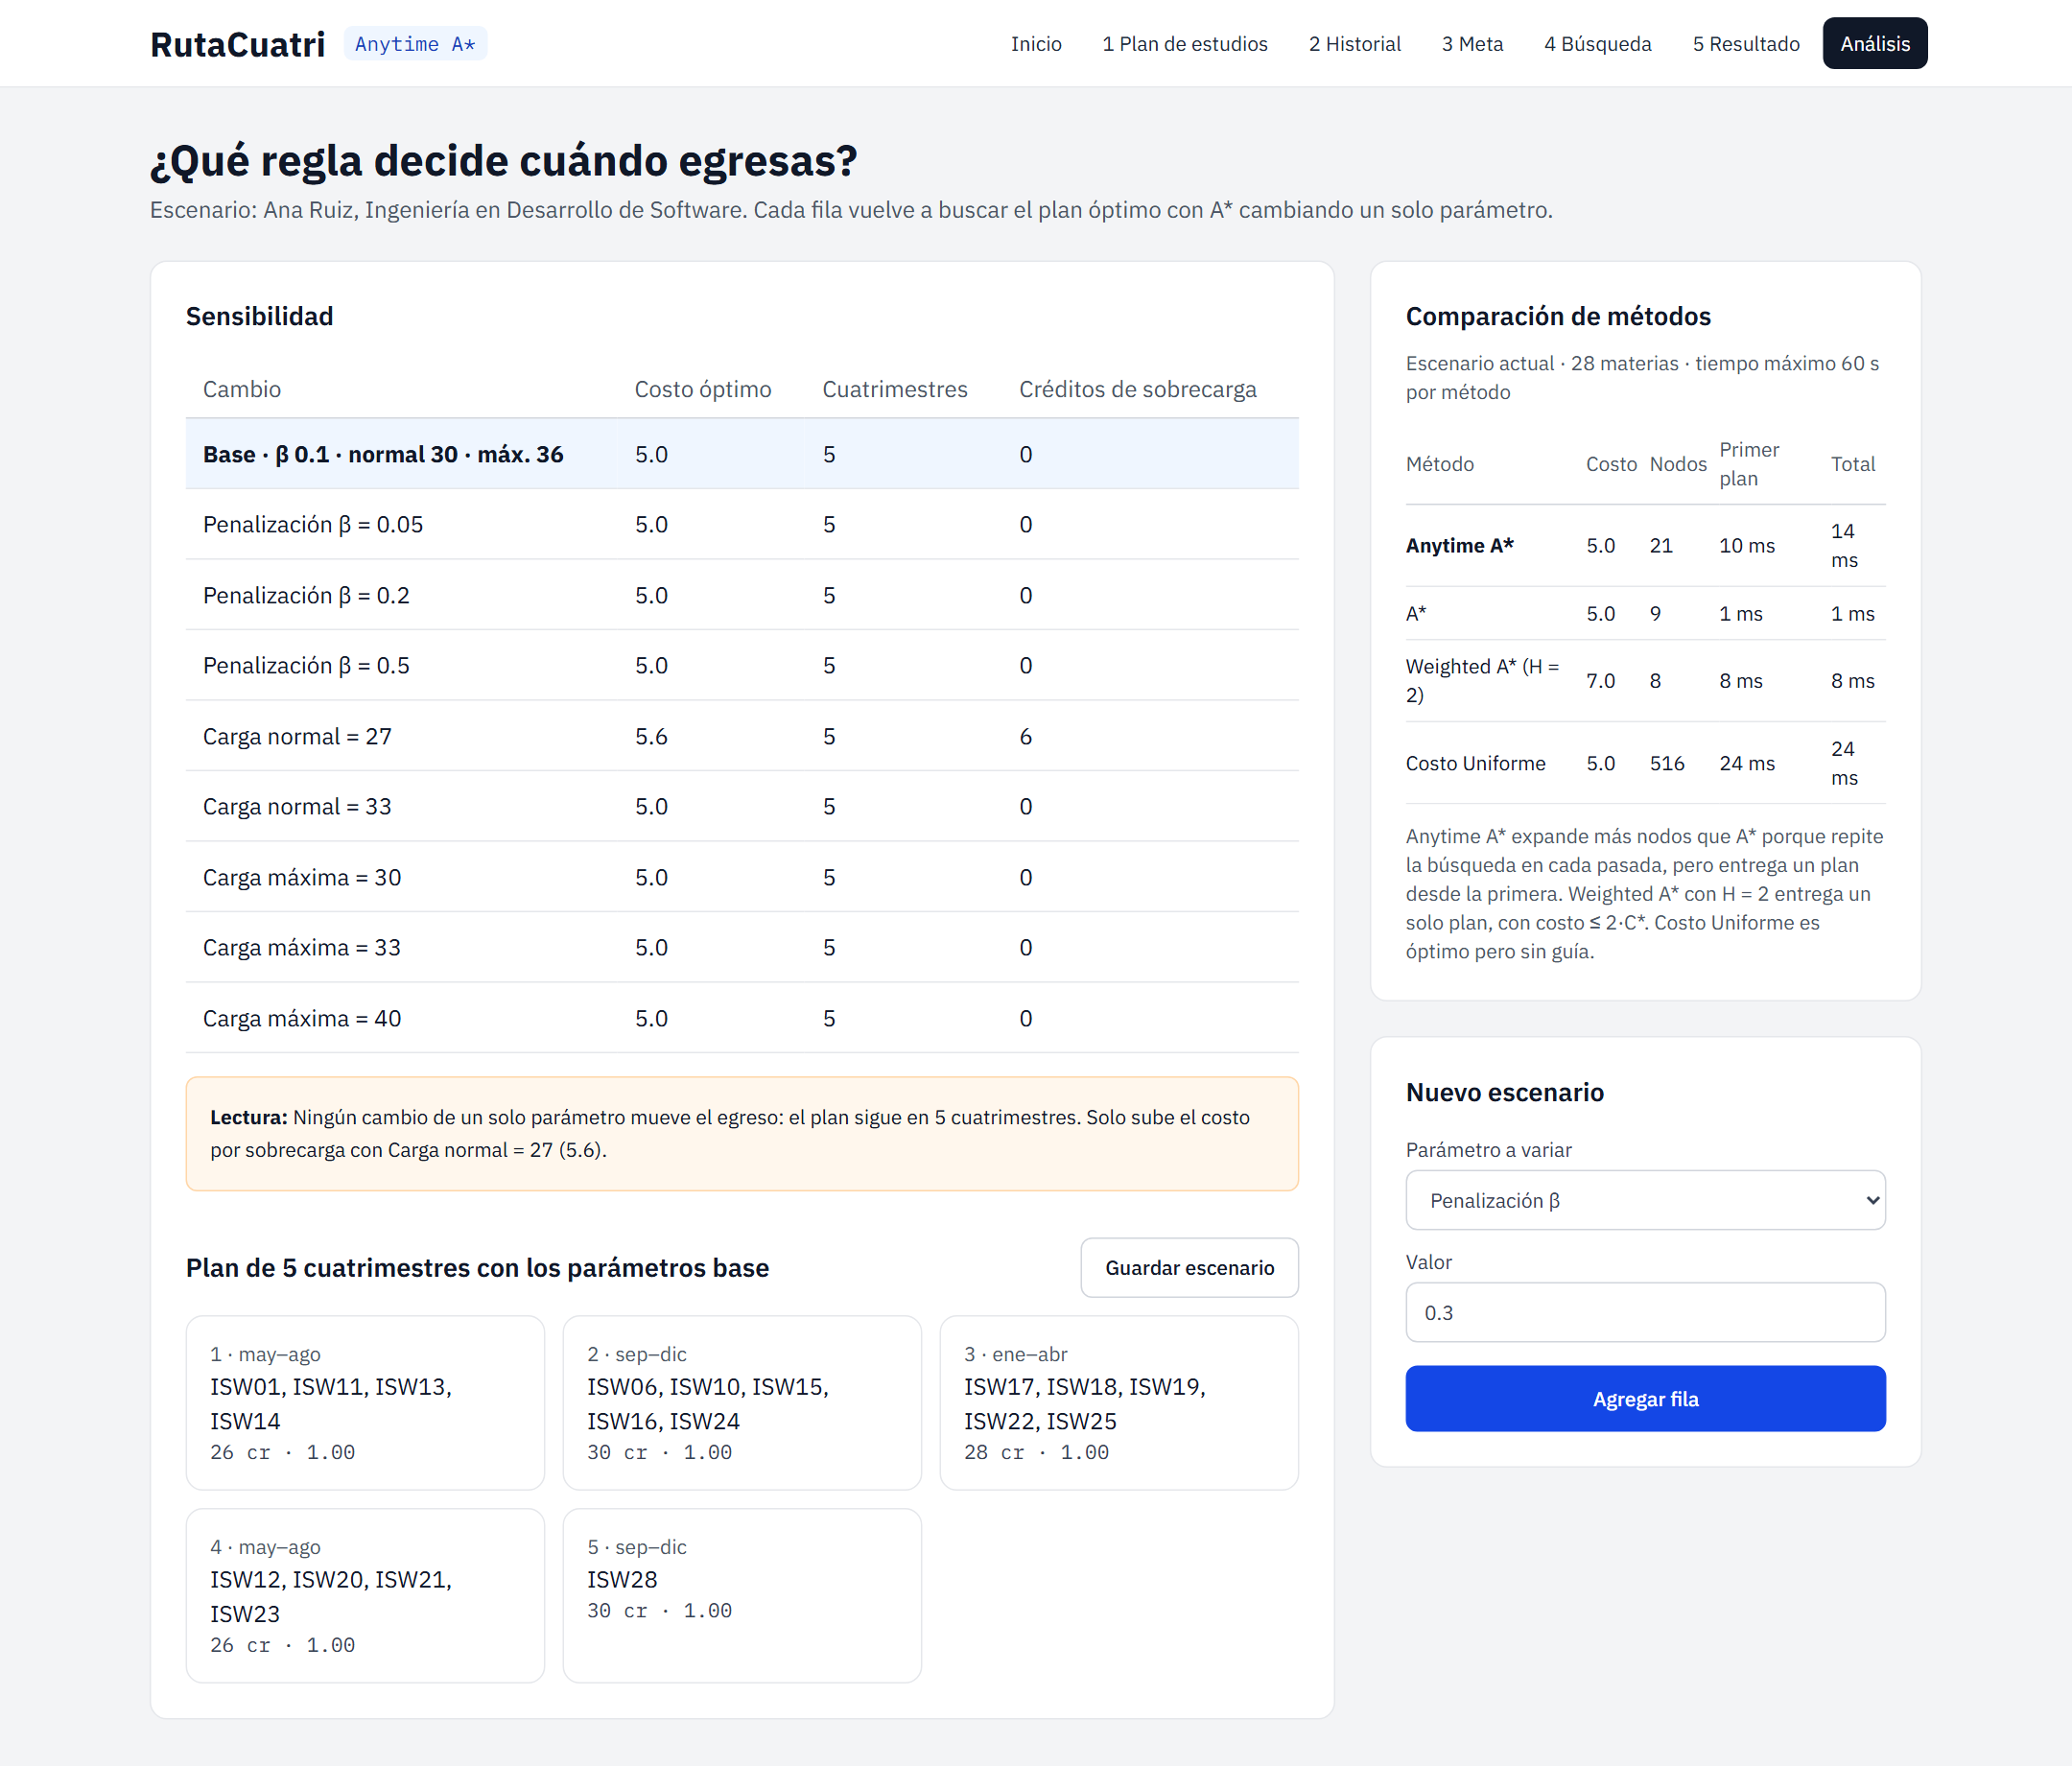
\includegraphics[width=\textwidth,height=0.8\textheight,keepaspectratio]{caso1-analisis}
    \caption{Pantalla de análisis de escenarios para el Caso 1}
    \label{FIG::Analisis}
\end{figure}

\section{Repositorio y ejecución}
\label{ANX::Repositorio}
El código está en \url{https://github.com/lsprz2773/RutaCuatri}. La Tabla~\ref{TAB::Carpetas} resume las carpetas y la Tabla~\ref{TAB::Comandos} los comandos; requiere Node 22.18 o superior.

\begin{table}[H]
  \begin{center}
    \caption{Carpetas del repositorio}
    \label{TAB::Carpetas}
    \begin{tabular}{|| p{5cm} | p{8.5cm} ||}
        \hline
        Carpeta & Contenido \\ [0.5ex]
        \hline\hline
        \texttt{src/motor} & Método de búsqueda (Capítulo 2) \\
        \hline
        \texttt{src/worker} & Web Worker que ejecuta el motor en el navegador \\
        \hline
        \texttt{src/app}, \texttt{src/componentes}, \texttt{src/estado} & Interfaz: las diez pantallas y su estado \\
        \hline
        \texttt{public/datos} & Las tres mallas, los alumnos tipo y las metas en JSON \\
        \hline
        \texttt{pruebas} & 77 casos de prueba, verificador, pruebas de propiedad y flujos de Playwright \\
        \hline
        \texttt{scripts} & Experimentos, implementación de referencia en Python y capturas \\
        \hline
        \texttt{resultados} & CSV de los experimentos A a D y datos del equipo \\
        \hline
    \end{tabular}
  \end{center}
\end{table}

\begin{table}[H]
  \begin{center}
    \caption{Comandos principales}
    \label{TAB::Comandos}
    \begin{tabular}{|| l | p{8cm} ||}
        \hline
        Comando & Qué hace \\ [0.5ex]
        \hline\hline
        \texttt{npm install} & Instala las dependencias \\
        \hline
        \texttt{npm run dev} & Abre la aplicación en \texttt{localhost:3000} \\
        \hline
        \texttt{npm test} & Corre las pruebas del motor \\
        \hline
        \texttt{npm run experimento} & Corre los experimentos A a D y escribe los CSV \\
        \hline
        \texttt{npm run build} y \texttt{npm run e2e} & Construye el sitio estático y corre Playwright \\
        \hline
    \end{tabular}
  \end{center}
\end{table}
